\documentclass[11pt, oneside]{article}   	
\usepackage{geometry}                		
\geometry{letterpaper}
\usepackage{graphicx}
\usepackage{qtree}
\usepackage{amssymb}

\setcounter{secnumdepth}{5}

\title{Homework 4}
\author{Abhi Agarwal}
\date{}					

\begin{document}
\maketitle
\section{Syntax-Directed Definitions}
\subsection{Question 1.1}

\subsubsection{Extend the SDD to handle division (``/'').} 

\begin{table}[h]
\begin{tabular}{lllll}
Production & Semantic Rule\\
L $\rightarrow$ $E_1$ \$ & L.val = $E_1$.val\\
E $\rightarrow$ $E_1$ + $T_2$ & E.val = $E_1$.val + $T_2$.val\\
E $\rightarrow$ $T_1$ & E.val = $T_1$.val\\
T $\rightarrow$ $T_1$ * $F_2$ & T.val = T1.val � F2.val\\
T $\rightarrow$ $T_1$ / $F_2$ & T.val = $T_1$.val / $F_2$.val\\
T $\rightarrow$ $F_1$ & T.val = $F_1$.val\\
F $\rightarrow$ ($E_1$) & F.val = $E_1$.val\\
F $\rightarrow$ digit & F.val = digit.lexval
\end{tabular}
\end{table}

\subsubsection{Draw the annotated parse tree for 3 + 8/2 \$.} 

\Tree [.L.val=7 [.E.val=7 [.E.val=3 [.T.val=3 [.F.val=3 digit.lexval=3 ] ] ] [.E.val=4 [.T.val=8 [.F.val=8 digit.lexval=8 ] ] [.F.val=2 digit.lexval=2 ] ] ] ]

\subsection{Question 1.2}
\par S-attributed and/or L-attributed

\subsubsection{For synthesized attribute $s$, and inherited attribute $i$:}

\par These rules are circular - it is not possible to evaluate either A.s node or B.i without evaluating the other and so we will see if they are S-attributed below.
\par S-attributed: The rules are S-attributed are that an SDD is S-attributed if every attribute is synthesized, and in this example this is not the case. A synthesized attribute at node N is defined only in terms of attribute values at the children of N and at N itself, but in the case of $A.s$ we are not seeing that. It's attribute values are referencing the ones of its parents, and so we rule out the fact that it can be S-attributed.  {\bf No} they are not S-attributed. The first rule defines an inherited attribute so they are automatically not S-attributed.
\par L-attributed: There is a cycle in the dependency graph here because we are referencing the first rule within the second rule, therefore it can't be L-attributed. Also the fact that A.s is to the right of C.s. {\bf No} it is not L-attributed.

\subsubsection{For synthesized attribute $z$ and given an externally defined scheme IfZero:} 

\par S-attributed: There are no inherited attributes. An SDD is S-attributed if every attribute is synthesized. Therefore, {\bf yes} this one is S-attributed.
\par L-attributed: Each attribute is synthesized as it is S-attributed. Nothing is inherited. We have to see if there are cycles in a dependency graph formed by these attributes in order to check if it is L-attributed. There seem to be no cycles in the dependency graph and therefore {\bf yes} it is L-attributed. 

\subsubsection{For inherited attribute $d$ and $a$ synthesized attribute $n$:} 

\par S-attributed: {\bf No} because this defines an inherited attribute $F_1$.d so the entire SDD cannot be S-attributed. Not everything is synthesized here.

\par L-attributed: {\bf Yes} it has elements which are either synthesized and follow the rules for proper inherited attributes, and there does not contain any cycles within it. 

\section{Syntax Directed Translation in Hacs}

\subsection{Question 2.1}

\par Output is T \& ! (F $|$ T)
\par This is because the bool.hx file we've passed into hacs is missing how to interpret the OR statement. The translation does not understand how to interpret $|$ and therefore it has left it as it was and outputted it in the same way to the user. It has recognized that there's an overuse of the brackets and therefore it has removed a pair of them. Because this is a AND statement the code can't interpret how to proceed and therefore just caries on. It also has left the NOT operation because it doesn't know what the $|$ and interprets it as something that can't be evaluated. 

\subsection{Question 2.2}
\par Here we fix the issue and we introduce the $|$ (OR) statement.
\\
\par root@debian:/home/abhi/Desktop/compiler\# \.\/Bool.run --sort=B --action=Evaluate --term='((T)\&!(F$|$T))' 
\par F 
\\
\par \noindent Below is the code that I wrote for it. Sorry I couldn't copy paste it in.
\par \noindent 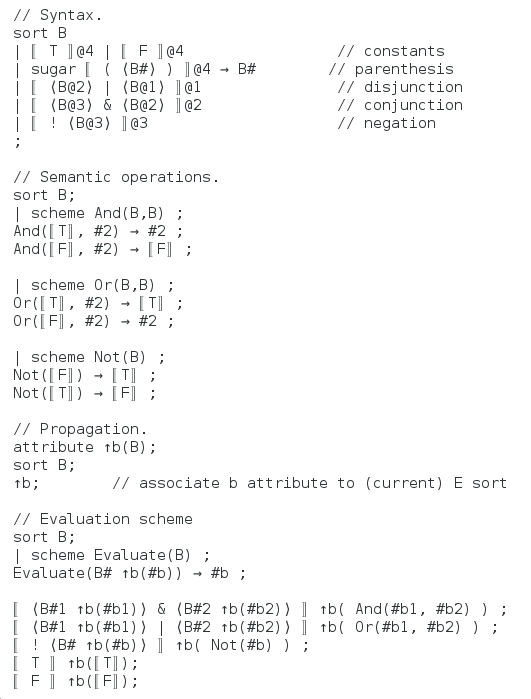
\includegraphics[scale=0.6]{hw1.png}
\end{document}  